%  TODO - Need oprn-field/maze cites with no reward
Exploration behavior can have two very different explanations depending on whether an animal might receive a reward. If there is no reason to expect a reward, exploration is treated as a search for information. We equate this with curiosity \cite{Berlyne1950,Schmidhuber1991,Kidd2015,Jaegle2019,Sumner2019,Calhoun2014,Wang2019,Auersperg2015}. For example, when a rat is placed in a novel environment it will explore, often extensivily, if no food and water is present, or expected \cite{Berlyne1950}. If reward is expected howeever exploration is interpreted as a search for reward \cite{Gupta2006,Sutton2018,Woodgate2017,Lee2011a,Schulz2018a,Calhoun2014}.

An open problem in the decision sciences it to unify exploration with exploitation, the policy of choosing the most rewarding action. This is union is difficult because exploration for reward has inhrently uncertain prospects. When it is combined with exploitation the conflict between them is irrational, which leads to the famous and fundamental exploration-exploitation dilemma \citep{Kelly1956,Berger-Tal2014,Dayan1996,Thrun1992,Mehlhorn2015,Kobayashi2019}, illustrated in Fig. \ref{fig:bee}a.

Our goal in this paper is to maximize the return of reward. Our goal is not to resolve the dilemma, fully. It is to find a way around it. We have come to believe curiosity, defined as learning for its own sake \cite{Loewenstein1994,Kidd2015,Gopnik2020}, is better general goal for exploration. This ``curiosity trick'', as we call it, is a counterintuitive suggestion. Why would it be better to search only to learn, instead of optimizing for reward? 

In this paper we will prove that exploration better handled by curiosity search even when the goal is to collect the most reward. We illustrate this view in Fig. \ref{fig:bee}b. We will prove this view offers a rational way around the dilemma. And we can justify our use of curiosity because it is a primary drive in most, if not all, animals \cite{Berlyne1950,Loewenstein1994,Inglis2001}. It is as strong, if not sometimes stronger, than the drive for reward \cite{Loewenstein1994,Kidd2015,Gottlieb2018,Sumner2019,Gopnik2020,Song2019,Wang2019}.

\begin{figure}
	\begin{fullwidth}
	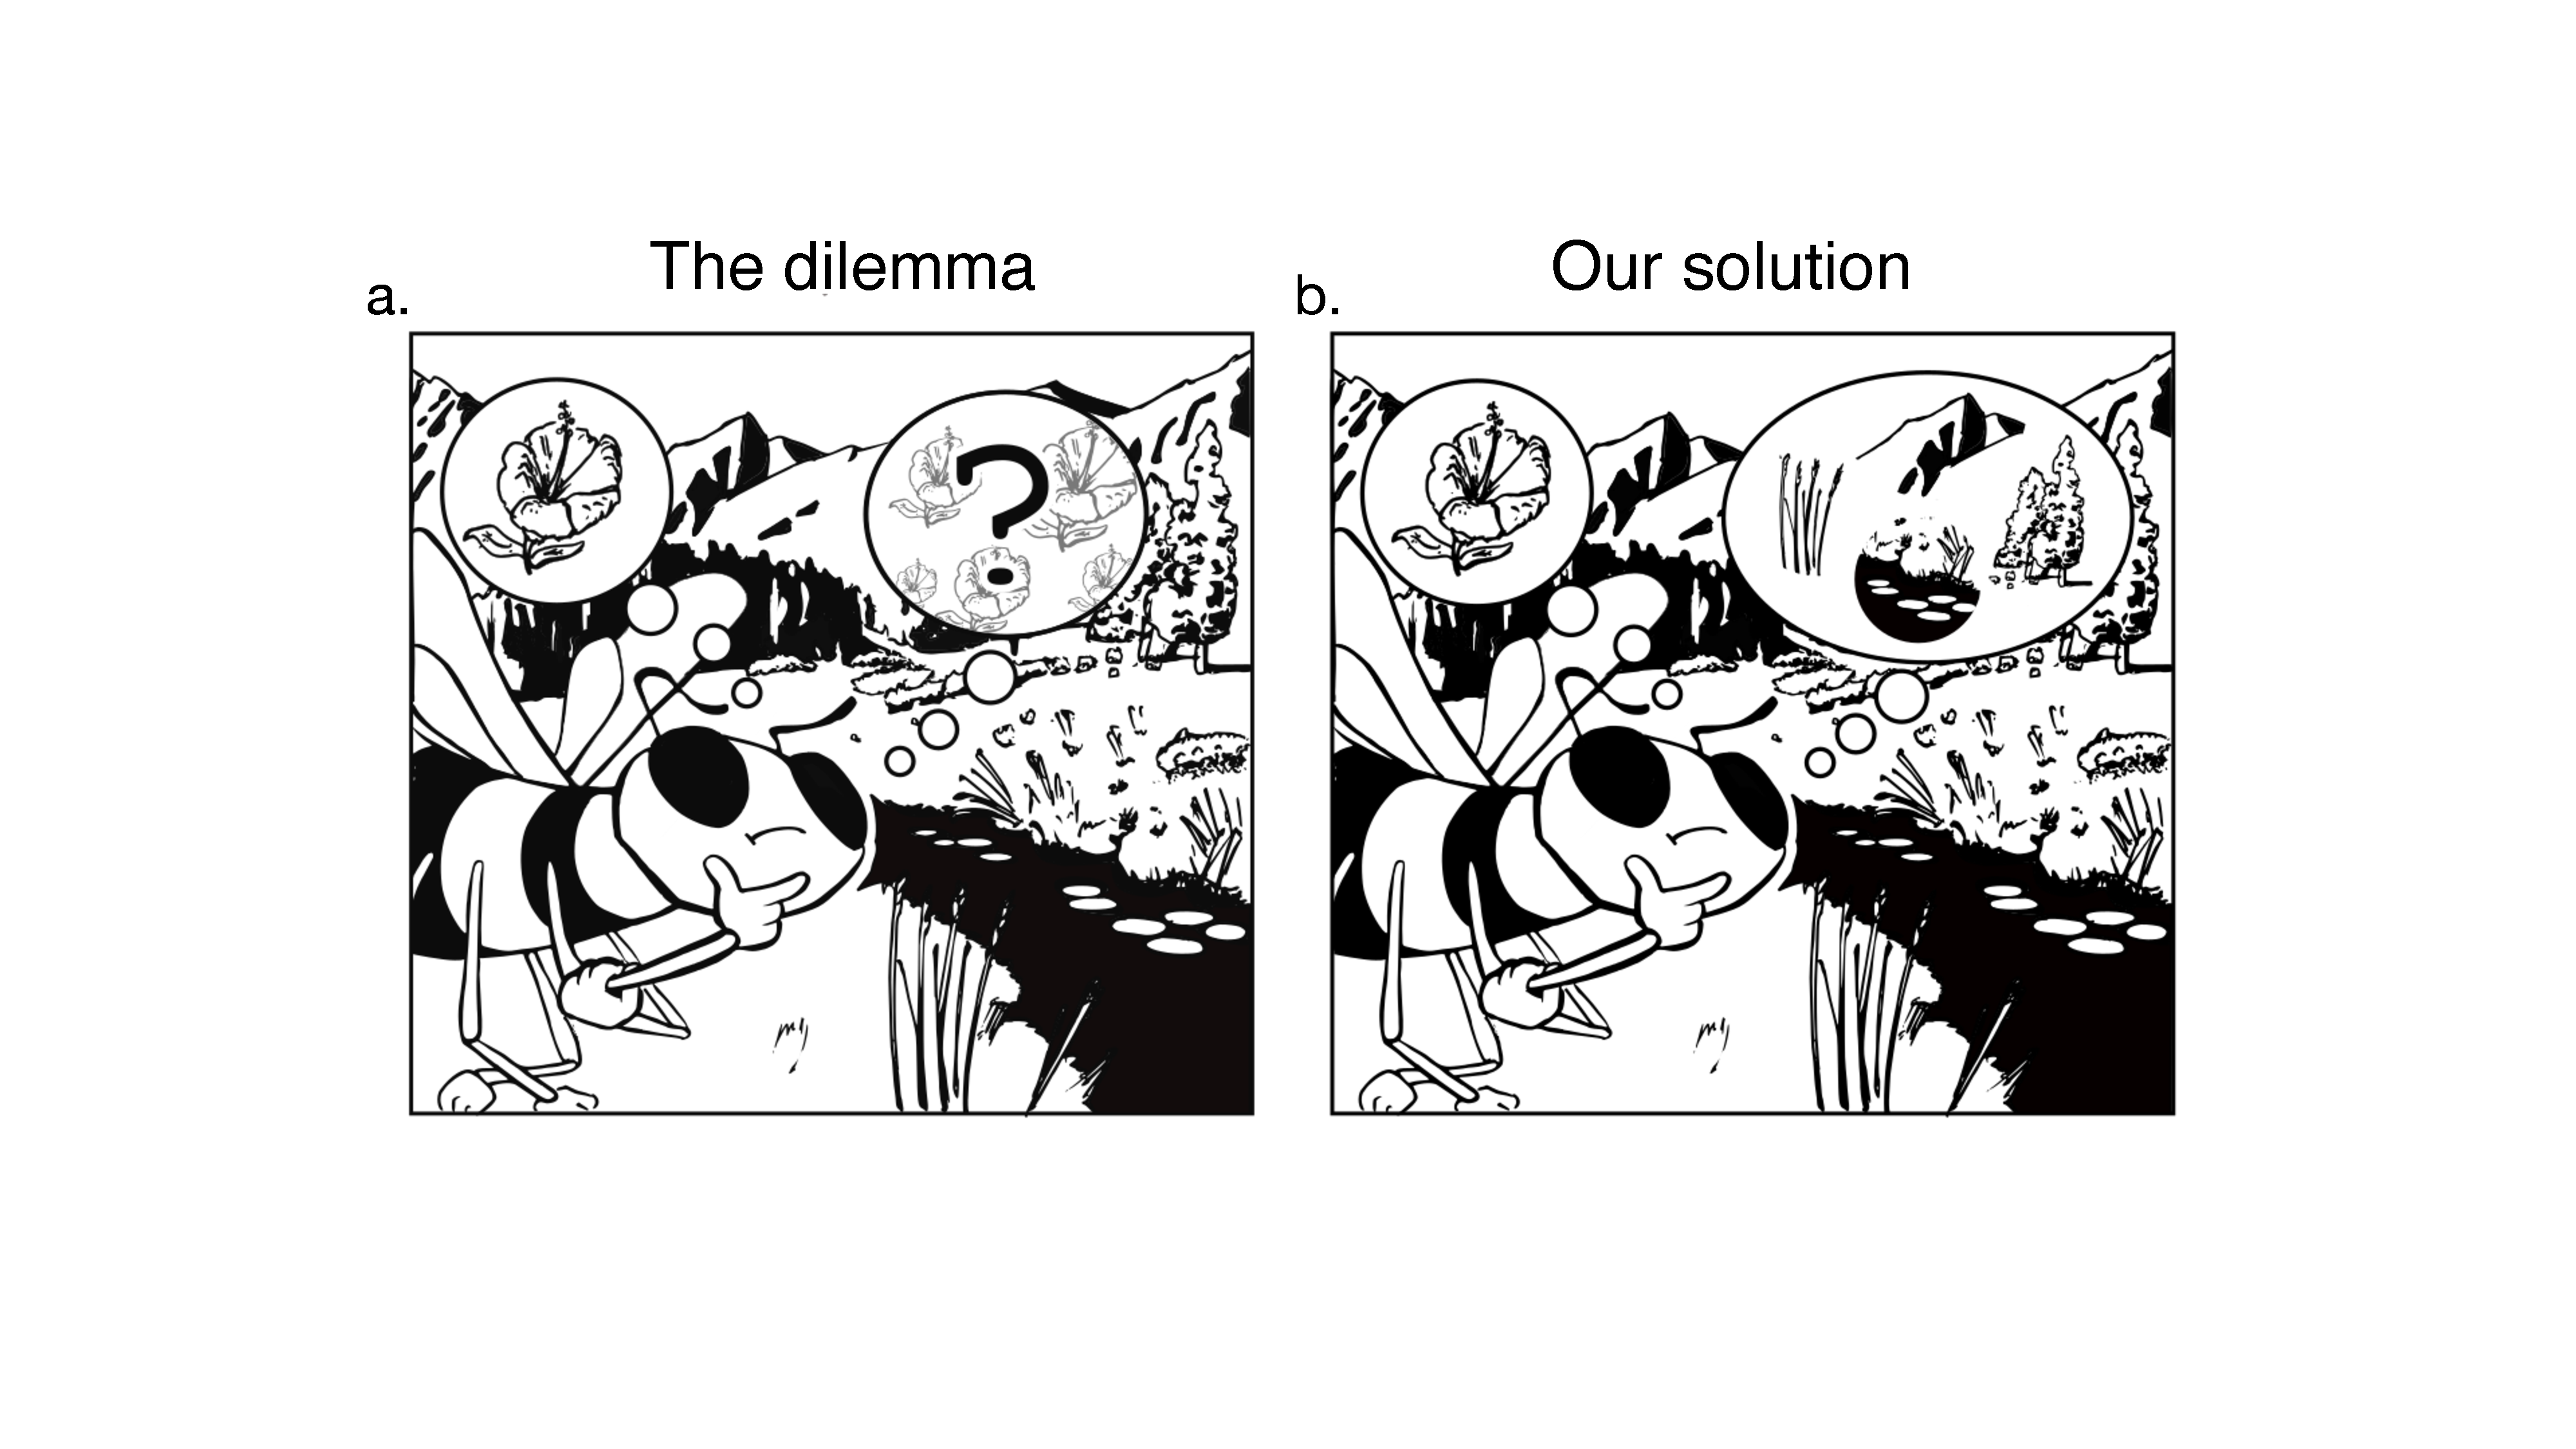
\includegraphics[width=.55\linewidth]{img/bee.pdf} 
	\caption{Two views of exploration and exploitation. \textbf{a}. The classic dilemma: either exploit an action with a known reward (e.g., return to the previous flower) or explore other actions on the chance they will return a better outcome. The central challenge here is that the outcome of exploration is uncertain, and filled with questions. \textbf{b}. An alternative view of the dilemma, with two goals: either maximize rewards \textit{or} maximize information value with a curious search of the environment. \textit{Artist credit}: Richard Grant.}
	\label{fig:bee} 
	\end{fullwidth}
\end{figure}

If exploration is just a search for information, then what was the dilemma can be divided into two problems. One problem is exploration (recast as a curious search). The other is exploitation, which still means a search for max reward. The focus of this paper is deriving a greedy and deterministic algorithm for solving both problems, simultaneously. We first develop a new mathmatical view of information value, curiosity, and a new understanding of ideal curious search. The second half uses these first results to prove our curiosity trick leads to an optimal value solution for nearly all explore-exploit decisions.

% When we observe an animal grappling with the decision to either explore or exploit, we often imagine this decision is based on reward. For example, if a bee goes in a familiar direction \textit{to gather nectar}, it is said to be exploiting past knowledge for environmental reward. If it goes in an unfamiliar direction \textit{to gather nectar}, it is said to be exploring for reward. Because the environment is partly unkown to the bee, it cannot rationally choose which action it should be doing, exploiting or exploring \textit{to gain more reward}. It is this uncertainty \textit{about returning the most rewards} that makes explore-exploit choices a dilemma. It is also this uncertainty which ensures there is no tractable mathematical solution for explore-exploit questions about reward \citep{Thrun1992a,Dayan1996,Ishii2002,Simsek2006,Gershman2018b}. We illustrate this view in Fig. \ref{fig:bee}a.

% The choice between exploring and exploiting is indeed faced routinely by learners of all kinds, including foraging bees, business organizations, humans, worms, monkeys, rodents, birds, children, and computer algorithms \citep{Gupta2006,Sutton2018,Woodgate2017,Lee2011a,Schulz2018a,Calhoun2014,Wang2019,Sumner2019,Auersperg2015}. But is reward really fundamental to it? Because in the natural world exploration already finds two explanations. If there is no reason to expect a reward, exploration is described theoretically as a search for information, what we will call curiosity \citep{Berlyne1950,Schmidhuber1991,Kidd2015,deAbril2018,Jaegle2019}. On the other hand, if reward is expected, then exploration gets re-interpreted as we described above, as a search for reward, and this specific interpretation is what leads the famous dilemma \citep{Kelly1956,Berger-Tal2014,Dayan1996,Thrun1992,Mehlhorn2015,Kobayashi2019}. 

% Why curiosity? Curiosity is a rational behavoir \cite{Rich2016a}, or so we argue. Curiousity is just as important for survival as reward collection \cite{Thrun1992}. Curiosity is a primary drive in most, if not all, animals \cite{Inglis2001}. It is as strong, if not sometimes stronger, than the drive for reward \cite{Loewenstein1994,Kidd2015,Gottlieb2018}. Curiosity, as an algorithm, is highly effective at solving optimization problems \cite{Schmidhuber1991,Pathak2017,Stanton2018,Lehman201,Mouret2011b1,Fister2019,Mouret2015,Colas2020,Cully2015,Pathak2017,Schwartenbeck2019.Laversanne-Finot2018}. In short, curiosity is necesssary, omnipresent, and effective.